\documentclass[../main.tex]{subfiles}
\begin{document}
Tutta la parte di Installazione dei Server è nei file allegati. In questo Capitolo andremo solo a vedere la parte di configurazione dei server. In questo capitolo ci sarà spesso una sovrapposizione dei server per l'istallazione quindi sarà importante leggere correttamente il nome del server su qui sono stati effettuati i lavori. 
\subsection{Configurazione Rete}
Dopo aver installato i due server la prima cosa da fare è impostare la rete su entrambi i server ma sopratutto di entrambe le schede di rete.
Come prima cosa ho impostato la rete NAT sul server lowsssva1 nel seguente modo

\subsubsection{NAT}
La rete che ho deciso di creare per la NAT è  la Nat 10.0.2.0/24 con i due server che hanno rispettivamente l'indirizzi seguenti .51 e .52  nel immagine possiamo vedere come è  stato configurato il server lowsssva1. Per quanto riguarda il server  lowsssva2 è  stato configurato in modo identico solo con il punto 52.


 \begin{figure}[h]
    \centering
    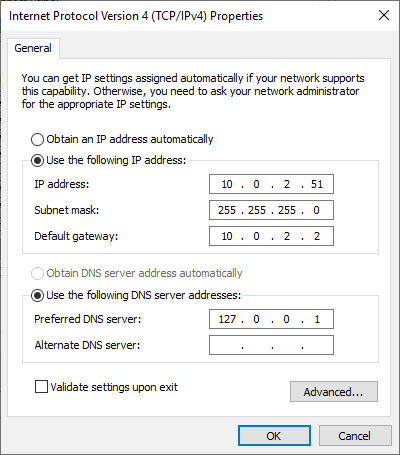
\includegraphics[width=0.5\textwidth]{Images/natServer1.PNG}
    \caption{Impostazioni NAT Server lowsssva1}
\end{figure}
\pagebreak{}
\thispagestyle{header-pages}

\subsubsection{Intranet}
Oltre che a una scheda di rete NAT i server sono stati dotati di un ulteriore scheda di rete, impostata in \textbf{Intranet}. Così da creare una rete private su qui impostare tutto il sistema. Le due schede sono state impostate in maniere leggermente diversa da un server all'altro. 
Come possiamo vedere la rete che ho deciso di creare in questo caso è la 10.20.0.0/24. Per quanto riguarda il primo server nel DNS fa un loopback della chiamata.


\begin{figure}[h]
  \centering
  \begin{minipage}[h]{0.4\textwidth}
    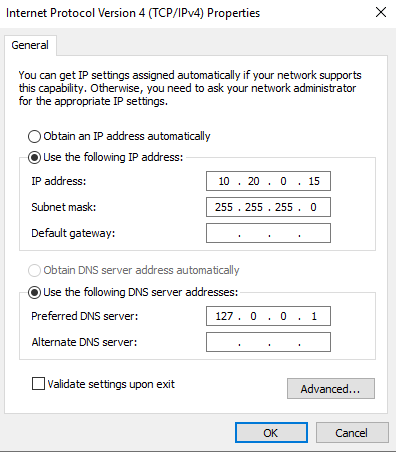
\includegraphics[width=\textwidth]{Images/intanetServer1.PNG}
    \caption{Impostazioni Intranet lowsssva1}
  \end{minipage}
  \hfill
  \begin{minipage}[h]{0.4\textwidth}
    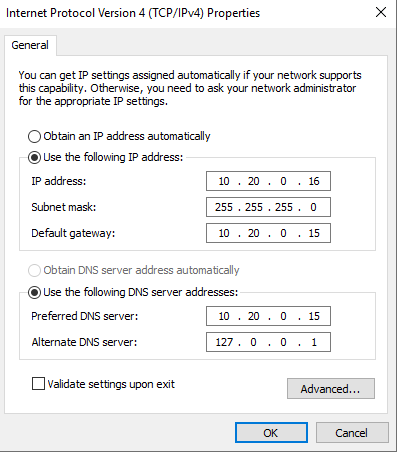
\includegraphics[width=\textwidth]{Images/intranet.PNG}
    \caption{Impostazioni Intranet lowsssva2}
  \end{minipage}
\end{figure}




\subsection{Configurazione Nome Server}
Per mettere i due server in dominio come prima cosa ho dovuto rinominare i server. Per fare questo mi sono recato nella schermata sottostante che è il server manager, ho cliccato sul nome attuale della macchina e ho cliccato il tasto \textbf{change}. Una volta che ho effettuato questo ho dovuto riavviare la macchina per fare in modo che il nuovo nome fosse applicato.

 \begin{figure}[h]
    \centering
    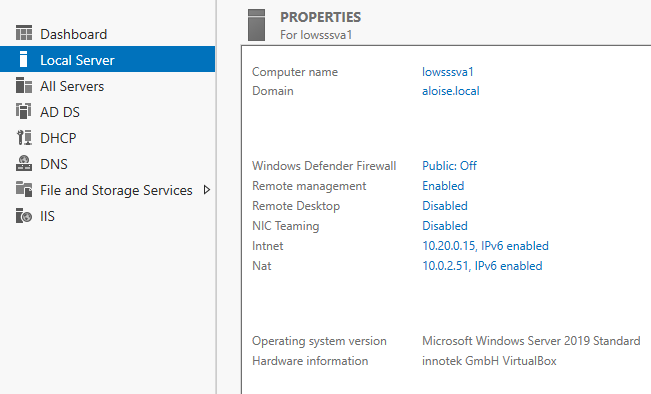
\includegraphics[width=0.5\textwidth]{Images/nomeServer.PNG}
    \caption{Cambio nome Server}
\end{figure}


\pagebreak{}
\thispagestyle{header-pages}

\subsection{Configurazione AD DS e DNS}

\subsubsection{Installazione}
Per configurare active directory e la sua ridondanza ho come prima cosa dovuto installarlo sul server lowsssva1.Vedi allegato Installazione ADDS.

Per installare e configurare ADDS sul server lowsssva2 le cose sono un po' diverse dalla configurazione base dato che ho dovuto collegare i due server. Come prima cosa ho dovuto installare il servizio andando sotto \textbf{Manage menu} e cliccare la voce \textbf{Add Roles and Features}.  Una volta fatto questo ho eseguito un installazione classica. Esattamente come quella effettuata sul server lowsssva1.

\subsubsection{Configurazione}
Per quanto riguarda la configurazione come dicevo poco sopra ho dovuto eseguire dei passaggi diversi dal primo server. Per Prima cosa ho dovuto non più creare una nuova foresta ma aggiungere il domain controler che stavo creando a un dominio esistente, come possiamo vedere dalla foto sottostante.


\begin{figure}[h]
    \centering
    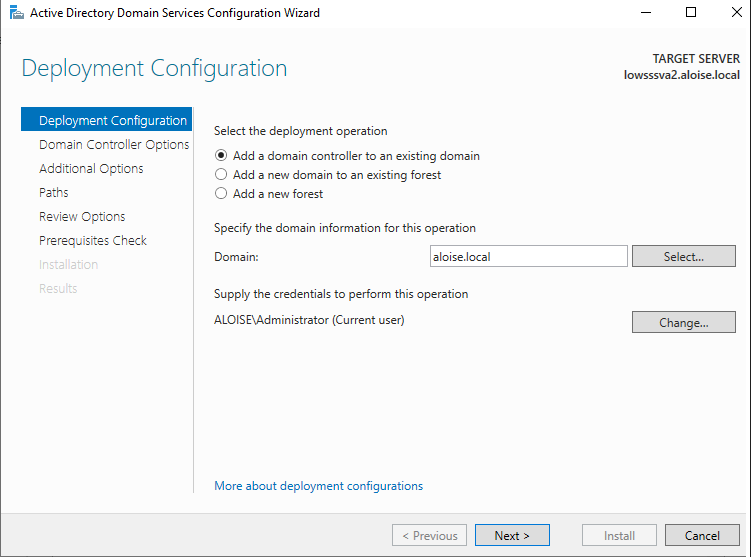
\includegraphics[width=0.75\textwidth]{Images/ad3.PNG}
    \caption{Domain controller e Foresta}
\end{figure}
\pagebreak{}
\thispagestyle{header-pages}

Una volta fatto questo sono andato avanti con la configurazione del ADDS e nella schermata seguente a quella appena visto ho lasciato tutto cosi, non ho dovuto mettere il visto sull'ultima voce seno il Domain controller che ho creato poteva solo leggere i dati e non modificarli. Ho inserito la Password e ho finito l'installazione, come ho anche detto nel file allegato nella schermata  dedicata a \textbf{SVSVOL} in un caso reale quei percorsi andrebbero cambiati e magari settati su un disco dedicato. 

\begin{figure}[h]
    \centering
    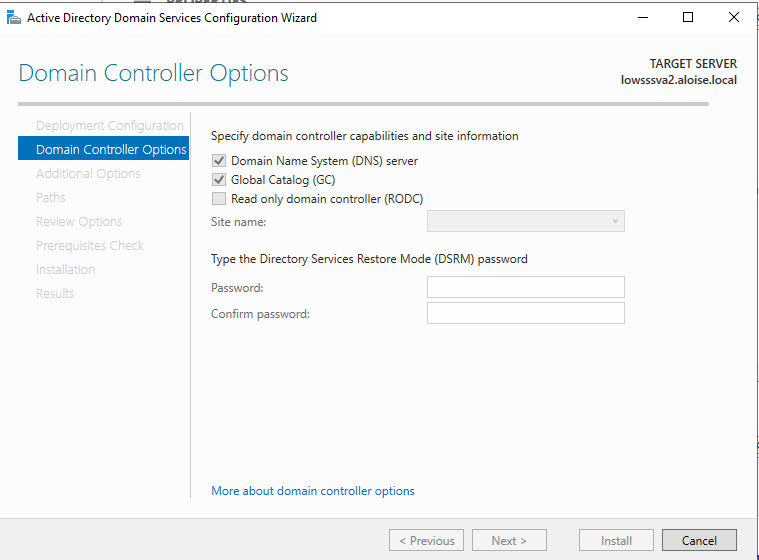
\includegraphics[width=0.75\textwidth]{Images/ad4.PNG}
    \caption{Domain controller e Foresta}
\end{figure}
Finita l'installazione il server lowsssva2 è correttamente inserito nel dominio e in completa ridondanza con il server lowsssva1.


\subsubsection{In passato }
In passato il DNS aveva una zona primaria e una zona secondaria, la particolarità era che era solo in lettura. Questo permetteva che il secondo server potesse solo rispondere alle richieste ma non poteva fare nessuna modifica in caso di bisogno.


\pagebreak{}
\thispagestyle{header-pages}

\subsection{Gestione Server}
Una delle cose richieste dal mandate era che i server fossero gestiti al meglio tramite i \textbf{tool manager} che Windows mette a disposizione. Per aderire a questa richiesta ho dovuto creare un account denominato \textit{sistemista} che avesse completo accesso al sistema che ho creato. Per fare questo ho dovuto prima di tutto installare Windows dopo di che rinominare la macchina e metterla in dominio. Dopo aver fatto tutto questo ho dovuto installare i tool mangar per gestire tutto in maniera corretta. Per fare questo ho dovuto cliccare \textbf{Manage menu} e dopo la voce  \textbf{add Server} una volta aggiunti tutti i server avremo la seguente schermata. In questo caso non tutti i server erano accessi come possiamo vedere.

\begin{figure}[h]
    \centering
    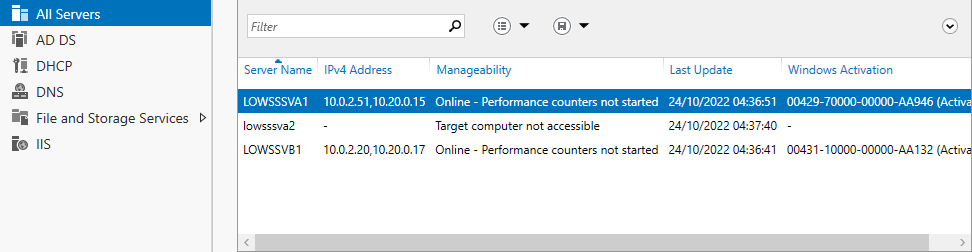
\includegraphics[width=0.6\textwidth]{Images/gestioneServer.png}
    \caption{Schermata di manger Server}
\end{figure}


\subsection{Configurazione DHCP}
\subsubsection{Installazione}
Per configurare il DHCP e la sua ridondanza ho come prima cosa dovuto installarlo sul server lowsssva1.Vedi allegato Installazione DHCP.

Per quanto riguarda l'installazione DHCP sul server lowsssva2 mi sono dovuto comportare come per il server lowsssva1.

\subsubsection{Configurazione}
Per quanto riguarda la configurazione della ridondanza del DHCP ho dovuto cercare online e dopo un po' di ricerche ho capito come comportarmi. Dopo aver impostato lo Scope DHCP di base sul server lowsssva1(Vedi guida) mi sono accorto che bastava andare sulla voce dello Scope e fare testo destro e cliccare la voce \textbf{failover} e seguire la configurazione guidata.


Qui di seguito si può trovare la configurazione che ho impostato. Come prima cosa dopo aver cliccato sul tasto detto poco sopra ci si apre questo pop-up dove mi è stato chiesto a che Scope volevo applicare il failover.

\begin{figure}[h]
    \centering
    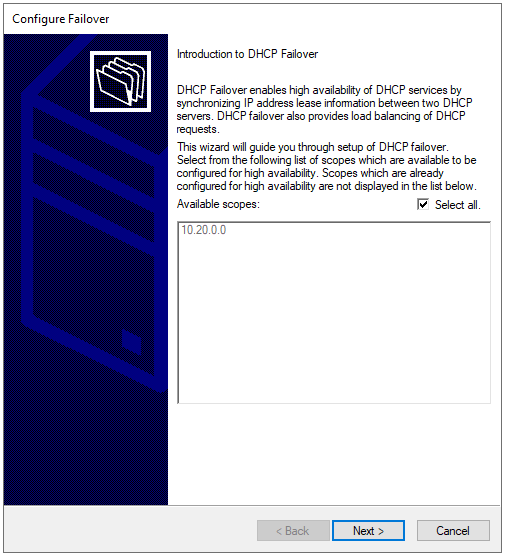
\includegraphics[width=0.25\textwidth]{Images/dhcp1.PNG}
    \caption{Set-up DHCP step 1}
\end{figure}


\pagebreak{}
\thispagestyle{header-pages}
Una volta cliccato questo ci basterà cliccare sul tasto per andare avanti.Una volta passati alla schermata successiva mi è stato chiesto con quale server volessi vare il failover, in questo caso ho scelto logicate il mio secondo server come possiamo notare dalla foto, cioè  lowsssva2.

\begin{figure}[h]
  \centering
  \begin{minipage}[h]{0.45\textwidth}
    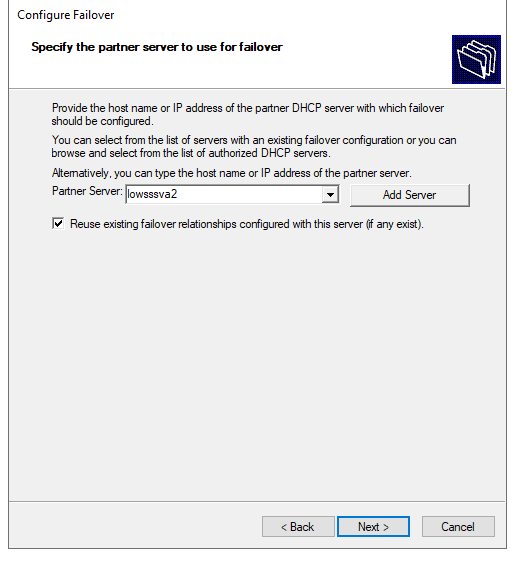
\includegraphics[width=\textwidth]{Images/dhcp2.PNG}
    \caption{Impostazioni Intranet lowsssva1}
  \end{minipage}
  \hfill
  \begin{minipage}[h]{0.45\textwidth}
    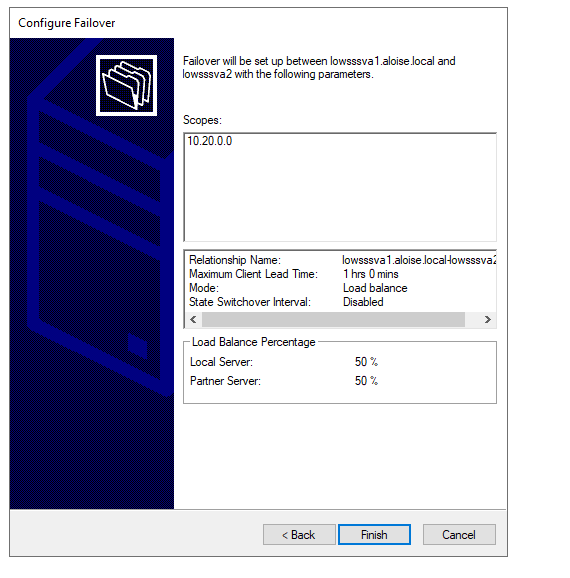
\includegraphics[width=\textwidth]{Images/dhcp3.PNG}
    \caption{Impostazioni Intranet lowsssva2}
  \end{minipage}
\end{figure}

Una volta fatto questo manca l'ultima parte quella più importante, quella della divisione del carico, in questo caso ho deciso di dividere il carico in modo equo trai due server.



\subsubsection{In passato }
In passato quando si impostava il DHCP failover, si impostava sul server principale al 80\% del lavoro mentre il secondo lo si impostava solo al 20\%.


\pagebreak{}
\thispagestyle{header-pages}
\subsection{Configurazione DFS}

\pagebreak{}
\thispagestyle{header-pages}
\subsection{Configurazione GPO}

In questo capitolo spiegherò quali regole ho imposto all'interno del mio dominio e perché ho scelto proprio queste regole. Oltre a questo vedremo anche come impostarle.

\subsubsection{Blocco al pannello di controllo}
\paragraph{Introduzione}
Trovo che la limitazione sull'accesso del pannello di controllo di un pc si molto importante per creare un ambiente di lavoro sicuro. Questo ci garantisce che nessun utente malintenzionato possa danneggiare la configurazione del nostro computer posto in dominio.


\paragraph{Configurazione}
Per poter impostare questa regola ho dovuto aprire in \textit{edit} la GPO creata per gli impiegati una volta fatto questo, sono andato sotto \textbf{User Configuration} dopo ho cliccato la voce \textbf{Administrative Templates} in fine \textbf{Control Panel} una volta arrivato qui ho cliccato la voce \textbf{Prohibit access to Control Panel and PC settings}, cliccata questa voce ci basterà cliccare \textbf{Enable} per rendere attiva questa regola.

\begin{figure}[h]
    \centering
    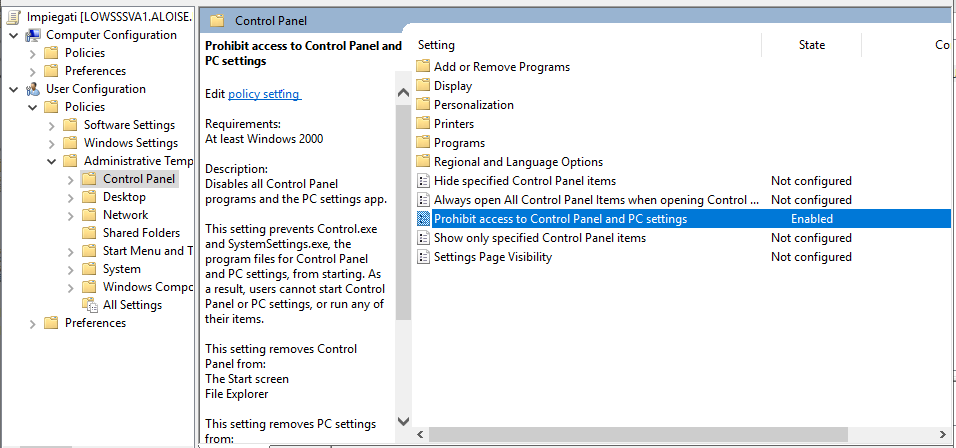
\includegraphics[width=1\textwidth]{Images/controlPanel.png}
    \caption{GPO Pannello di controllo}
\end{figure}
\pagebreak{}
\thispagestyle{header-pages}

\subsubsection{Controllare l'accesso al prompt dei comandi}
\paragraph{Introduzione}
I prompt dei comandi possono essere utilizzati per eseguire comandi di alto livello e così facendo si rischia di eludere alcune restrizioni sul sistema impostate dal gestore della rete, ecco perché ho deciso di disabilitare questa possibilità. Dopo aver abilitato questa regola se qualcuno tenta di accedere al CMD gli apparirà un messaggio dove viene detto che alcune impostazioni sono bloccate.



\paragraph{Configurazione}
Per poter impostare questa regola ho dovuto aprire in \textit{edit} la GPO creata per gli impiegati una volta fatto questo, sono andato sotto \textbf{User Configuration} dopo ho cliccato la voce \textbf{Administrative Templates} in fine in \textbf{System} una volta arrivato qui ho cliccato la voce \textbf{Prevent access to the command prompt} cliccata questa voce ci basterà cliccare \textbf{Enable} per rendere attiva questa regola.


\begin{figure}[h]
    \centering
    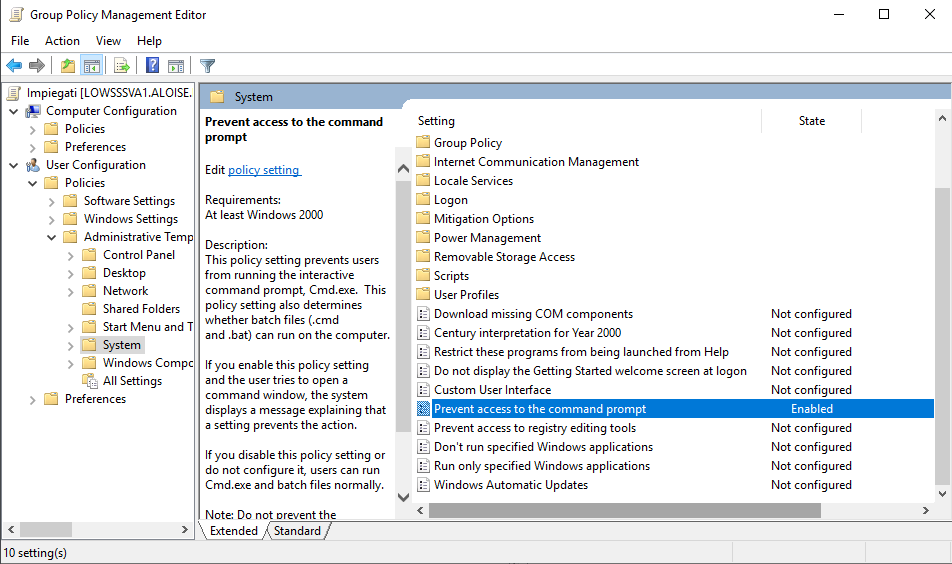
\includegraphics[width=1\textwidth]{Images/CmdBlocco.png}
    \caption{GPO Cmd blocco}
\end{figure}

\pagebreak{}
\thispagestyle{header-pages}

\subsubsection{Riavvio forzato del sistema disabilitato}

\paragraph{Introduzione}
Questa regola non è tanto per la sicurezza del computer in sé ma più per la sicurezza dell'utente che sta lavorando per evitare spiacevoli inconvenienti. Esempio stati lavorando sul computer e Windows visualizza un messaggio che indica che il tuo sistema deve essere riavviato a causa di un aggiornamento. Se non si è veloci a leggere il messaggio e rispondere il pc si riavvia in automatico e questo fa perdere magari tutto il lavoro svolto sui file.


\paragraph{Configurazione}
Per poter impostare questa regola ho dovuto aprire in \textit{edit} la GPO creata per gli impiegati una volta fatto questo, sono andato sotto \textbf{Configurazione computer} dopo ho cliccato la voce \textbf{Administrative Templates}in fine in \textbf{Windows Update}na volta arrivato qui ho cliccato la voce \textbf{No auto-restart with logged on users for scheduled automatic updates installations} cliccata questa voce ci basterà cliccare \textbf{Enable} per rendere attiva questa regaola.

\begin{figure}[h]
    \centering
    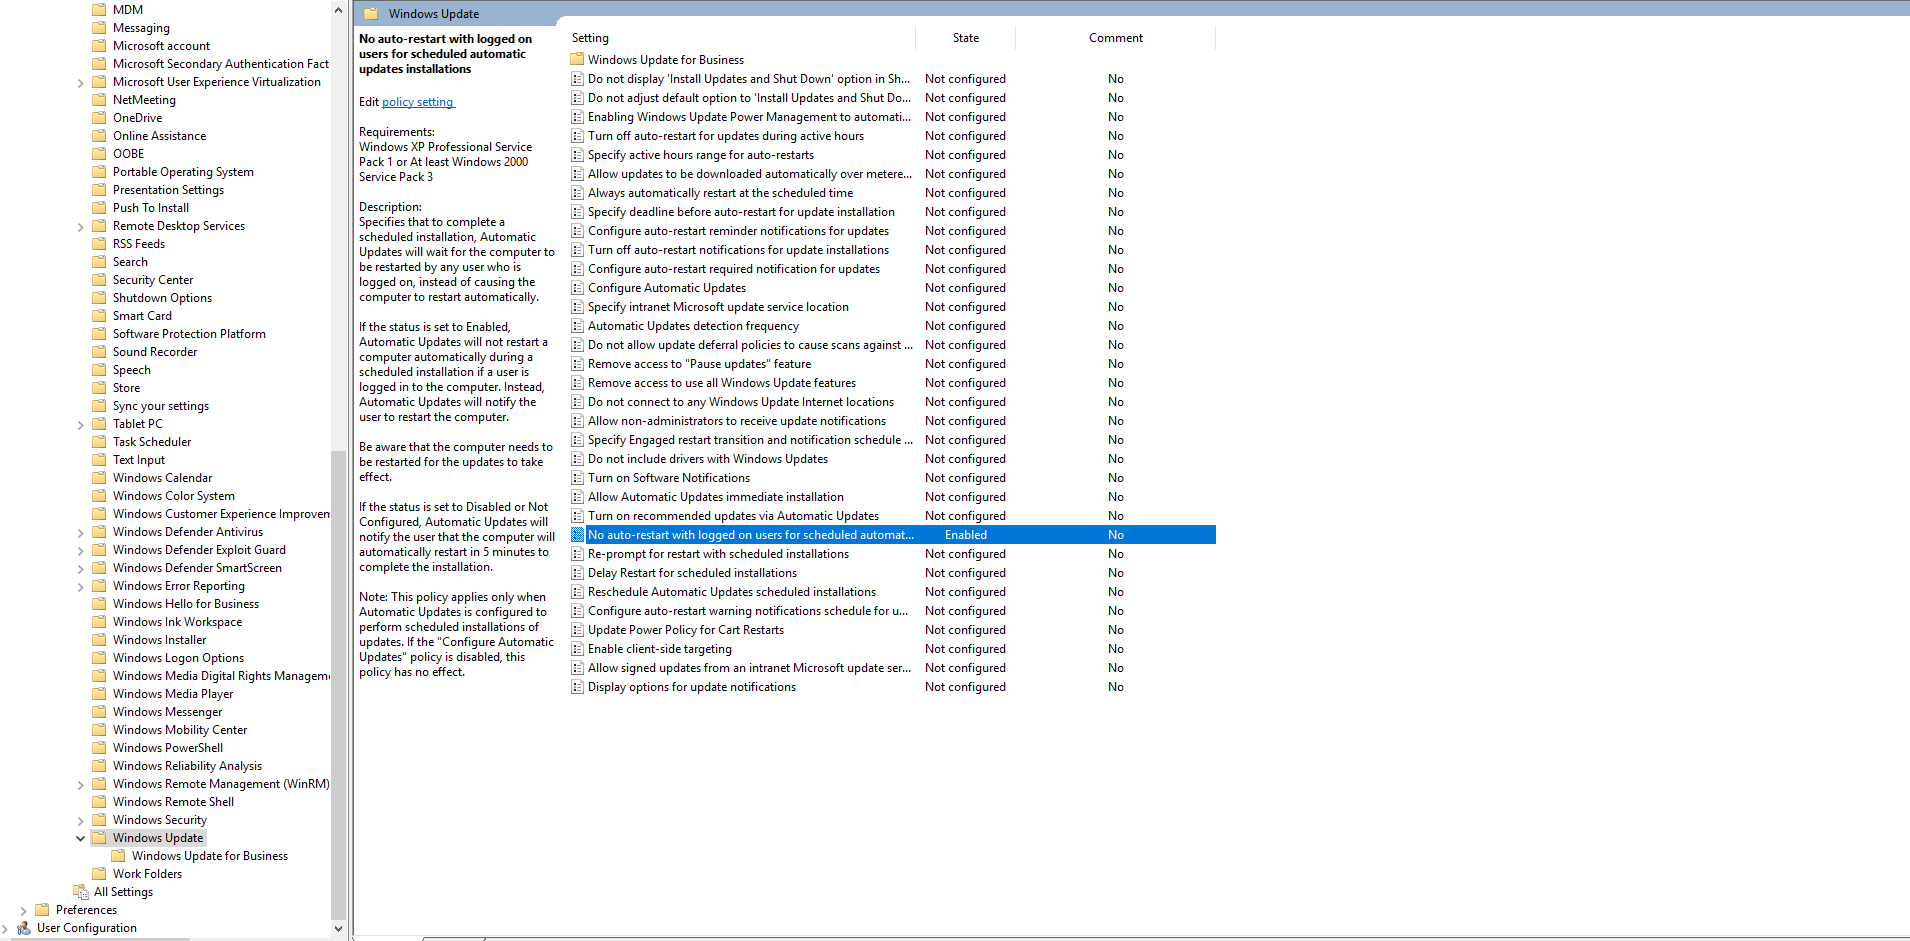
\includegraphics[width=1\textwidth]{Images/bloccoRiavvio.png}
    \caption{GPO Riavvio forzato bloccato}
\end{figure}


\pagebreak{}
\thispagestyle{header-pages}
\subsubsection{Limita le installazioni di software}
\paragraph{Introduzione}
Dando la possibilità agli utenti di installare programmi si rischia moltissimo, sia da programmi indesiderati che potrebbero persino rovinare la configurazione del pc che si trova in dominio. Per questo devono essere solo gli amministratori a poter installare un programma e hanno anche il compito di eseguire la manutenzione e pulizia ditali programmi.

\paragraph{Configurazione}
Per poter impostare questa regola ho dovuto aprire in \textit{edit} la GPO creata per gli impiegati una volta fatto questo, sono andato sotto \textbf{Computer Configuration} dopo ho cliccato la voce \textbf{Administrative Templates} poi ho cliccato la voce \textbf{Windows Component} e in fine \textbf{Windows Installer} una volta arrivato qui ho cliccato la voce \textbf{Prohibit User Install} cliccata questa voce ci basterà cliccare \textbf{Enable} per rendere attiva questa regola.

\begin{figure}[h]
    \centering
    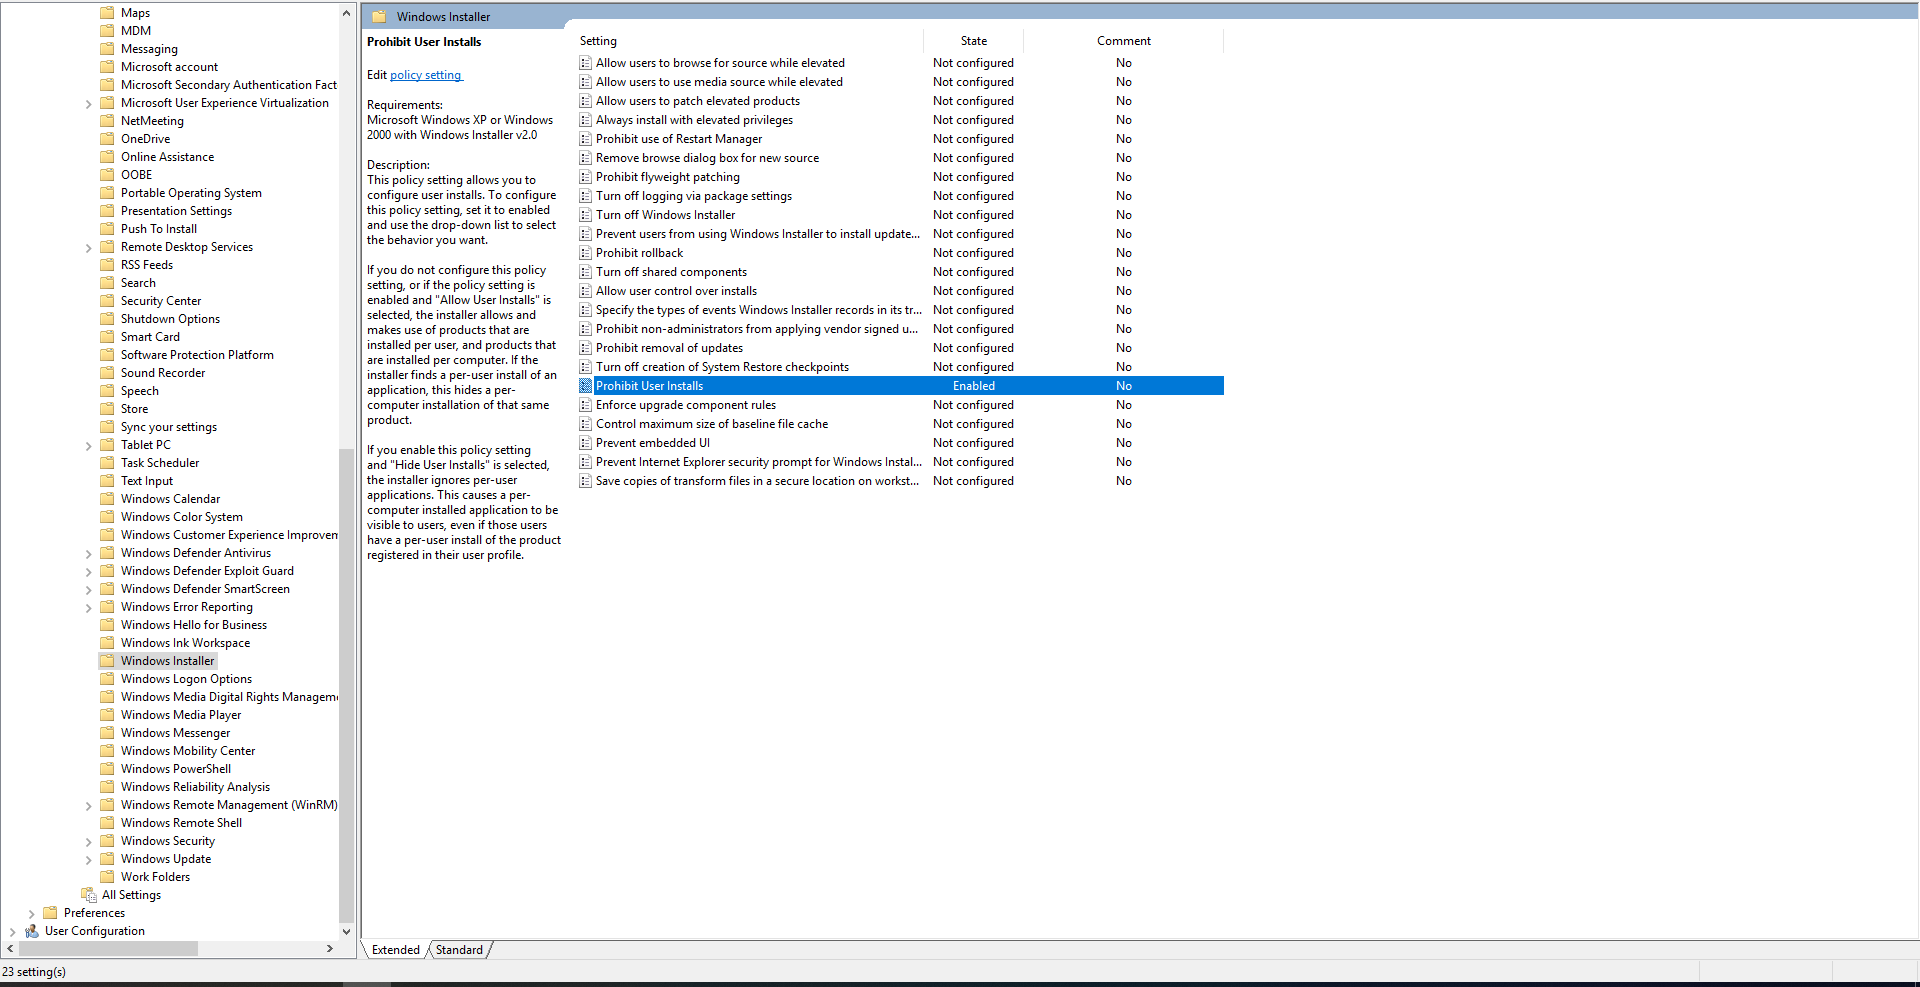
\includegraphics[width=1\textwidth]{Images/BloccoProgrammi.png}
    \caption{GPO blocco Programmi}
\end{figure}

\pagebreak{}
\thispagestyle{header-pages}

\subsubsection{Disabilita l'Account Ospite}
\paragraph{Introduzione}
Con un account ospite gli utenti hanno accesso a dati sensibili. Dato che questi account concedono l'accesso al pc senza alcuna password. Lasciare sbloccato la possibilità di fare login con questi account significa esporre un grande pericolo il computer di dominio. Di default questa regola è già attiva.

\paragraph{Configurazione}
Questa regola a differenza di tutte le altre era già attiva, ma per controllare che lo fosse davvero ho dovuto eseguire i segenti passaggi, ho dovuto aprire in \textit{edit} la GPO creata per gli impiegati una volta fatto questo, sono andato sotto \textbf{Computer Configuration} dopo ho cliccato la voce \textbf{Windows Settings} poi ho cliaccato la voce \textbf{Security Settings} e in fine \textbf{Security Options} una volta arrivato qui ho cliccato la voce \textbf{Accounts: Guest Account Status} cliccata questa voce ho semplicemnte controllato che fosse già \textbf{Disabled}

\begin{figure}[h]
    \centering
    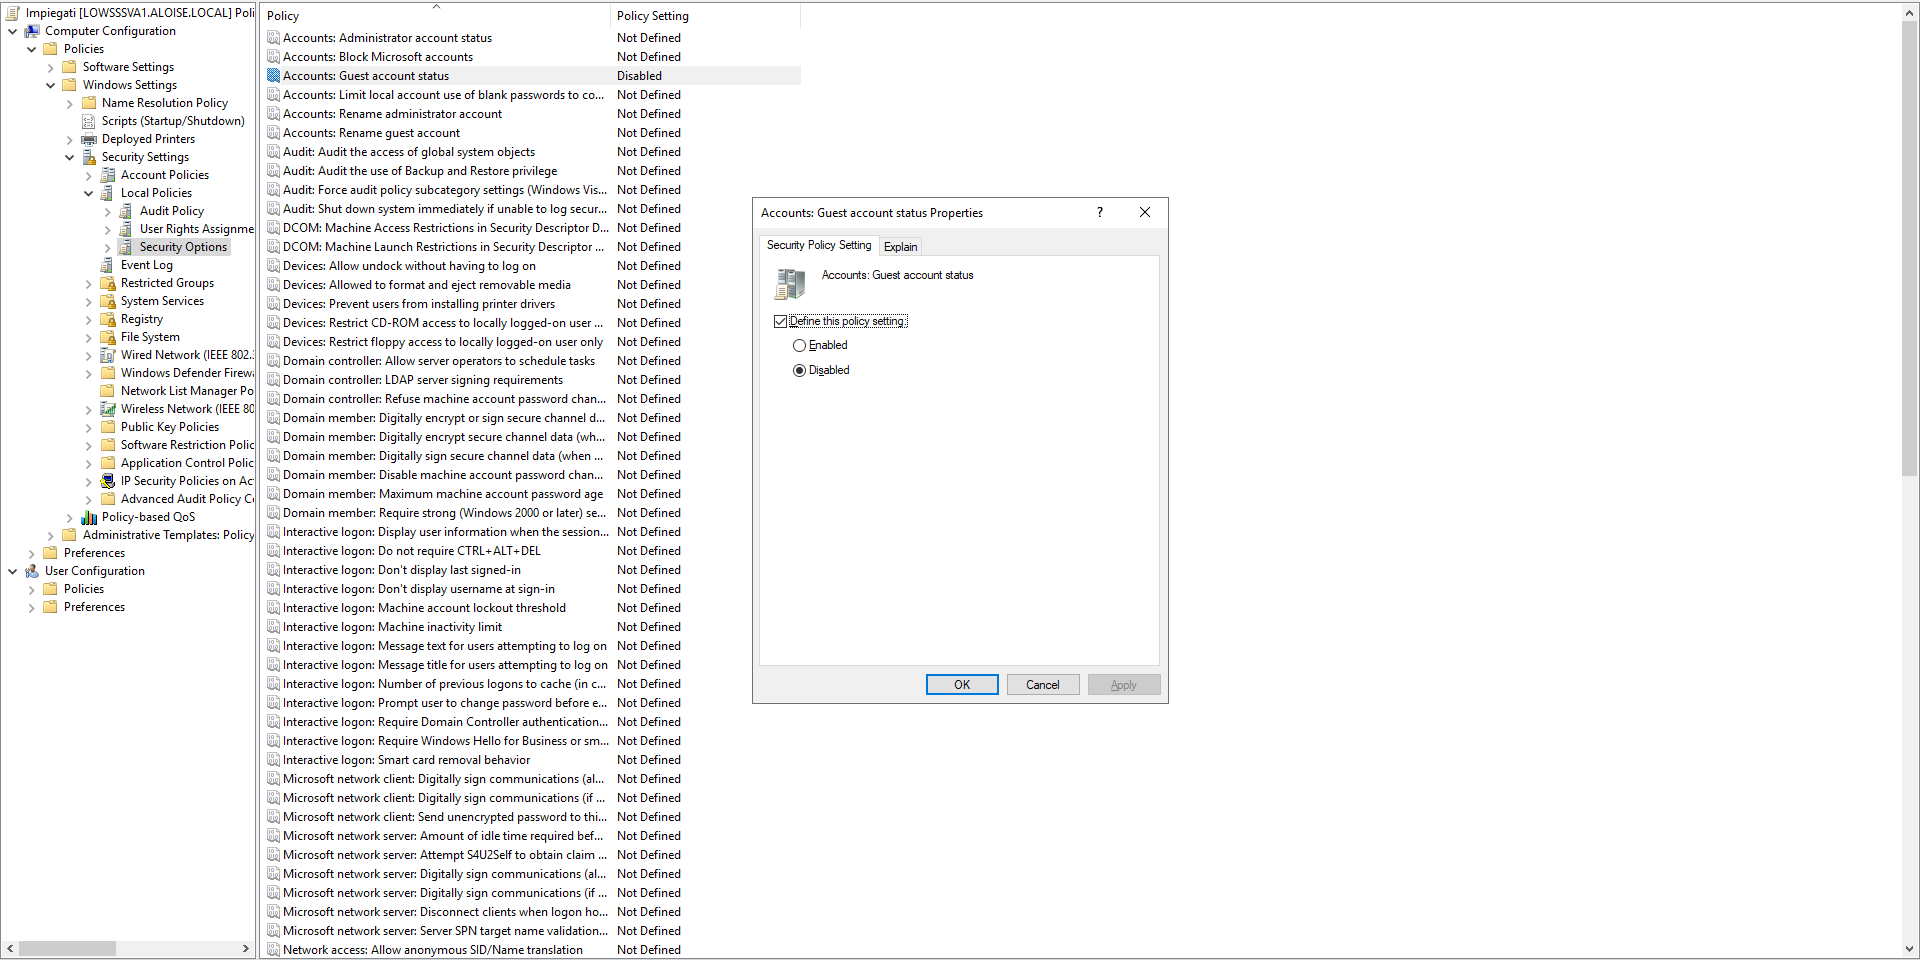
\includegraphics[width=1\textwidth]{Images/ospite.png}
    \caption{GPO blocco account ospite}
\end{figure}

\pagebreak{}
\thispagestyle{header-pages}
\subsubsection{Imposta la lunghezza minima della password su limiti superiori}
\paragraph{Introduzione}
Impostare delle regole per le password è molto importante per la sicurezza degli utenti. Esempio per un utente di alto livello si predilige una password con più caratteri e quindi più robusta con magari 15 caratteri. Mentre per un account normale magari solo 12 caratteri. In questo caso il valore di default è 0 quindi bisogna per forza impostare una regola per tenere il dominio protetto in maniera corretta.

\paragraph{Configurazione}
Per andar a modificare il valore di default ho dovuto fare i seguenti passaggi. Ho dovuto aprire in \textit{edit} la GPO creata per gli impiegati una volta fatto questo, sono andato sotto \textbf{Computer Configuration} dopo ho cliccato la voce \textbf{Windows Settings} poi ho cliccato la voce \textbf{Security Settings} e in fine \textbf{Account Policies} una volta arrivato qui ho cliccato la voce \textbf{Minimum password length} cliccata questa voce ho semplicemente inserito la lunghezza minima che volevo per la password e ho cliccato \textbf{Apply}


\begin{figure}[h]
    \centering
    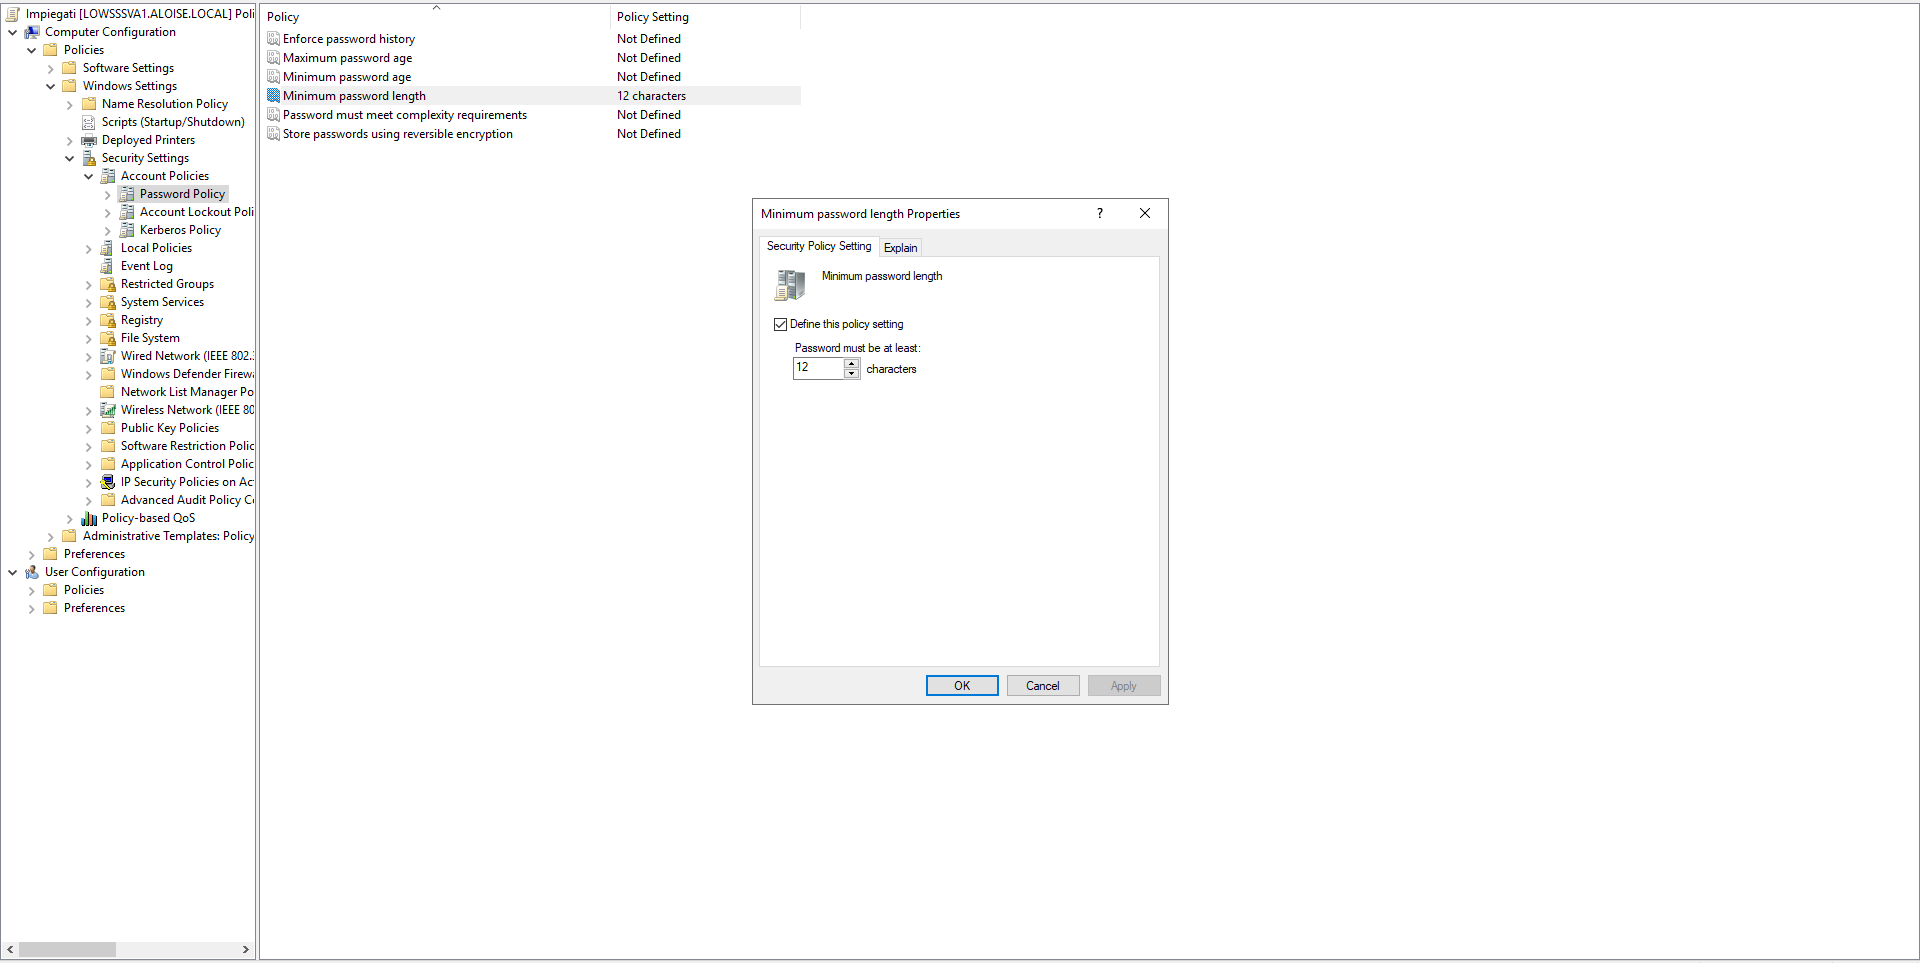
\includegraphics[width=1\textwidth]{Images/Password.png}
    \caption{GPO lunghezza minima password}
\end{figure}

\end{document}  
